\documentclass{article}
\usepackage{dingbat}
\usepackage{tikz}
\usetikzlibrary{positioning}
\usetikzlibrary{shapes.geometric}
\usetikzlibrary{shapes.symbols}
\usetikzlibrary{shadows}
\usetikzlibrary{arrows}

\pagestyle{empty}

\begin{document}

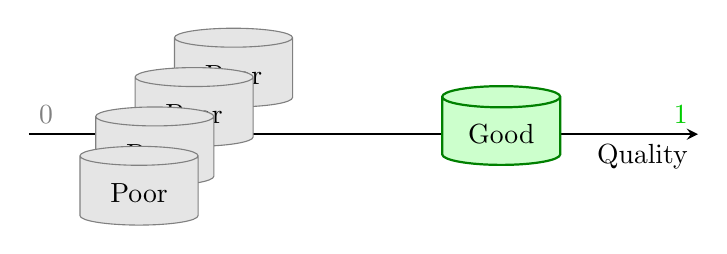
\begin{tikzpicture}
	[basket/.style={cylinder, shape border rotate=90,aspect=0.25, minimum height=1cm,minimum width=1.5cm},
	poor/.style={basket, draw=gray, fill=gray!20!white},
	good/.style={basket, thick, draw=green!50!black, fill=green!20!white}]

\draw [->,thick,draw=,>=stealth] (-2,-0.75) node [above right,gray] {0} -- (6.5, -0.75) node [above left,green!80!black] {1} node [below left,black] {Quality};
\node [poor] at (0.6,0.0) {Poor};
\node [poor] at (0.1,-0.5) {Poor};
\node [poor] at (-0.4,-1.0) {Poor};
\node [poor] at (-0.6,-1.5) {Poor};
\node [good] at (4,-0.75) {Good};

\end{tikzpicture}
\end{document}
